\chapter{A Physical Perspective on The Rescue of Mutant CFTR}
\label{chap:perspective}

\begin{chapquote}{Deborah Marcus \cite{marcus_ouroboros}}
and take the time to remember\\
the looping bend, surged\\
began as the walking end
\end{chapquote}

\section{Introduction}

The preceding chapters have fit into some broad themes. Chapters \ref{chap:introduction} and \ref{chap:methods} outlined a philosophy of biological physics. Meanwhile, chapters \ref{chap:cftr}-\ref{chap:opening} collected molecular details about the misfunction of CFTR, to built up an understanding of the root cause of Cystic Fibrosis, and demonstrate that small molecule drugs can rescue diverse modes of CFTR misfunction. In this chapter we will tie these themes together. We will introduce a physical perspective on the rescue of mutant CFTR by potentiator drugs. A similar model could be built for corrector drugs, or even used to think about the modulation of any protein by small molecules.

We hope that this model will inform our current understanding of the action of CFTR modulators and also direct future efforts in treating the root cause of Cystic Fibrosis. We will outline specific studies motivated by this model in the next chapter.

We will begin with a brief overview of our results so far, analysing 4 rare CF-causing mutations which appear to respond to CFTR modulators even though they each have a unique molecular defect. We will then look at the molecular details of one of the best studied and most common disease causing mutations, G551D

%, and where it fits in relation to the array of other disease causing mutations. 

We will show through simple unbiased MD, that this mutation causes a disruption to the binding of ATP, resulting in a gating defect. As with previous chapters, this gating defect appears unique, sharing little in common with the other gating defects we analysed previously. This array of different disease phenotypes leads us to propose a model based on the gating energy landscape, which accounts for the rescue of unique phenotypes by a common mechanism of action. 

We will demonstrate how to use our proposed model to theratype a rare mutation, Q1291H, from the molecular level. We will show how the Q1291H mutation appears to exhibit a similar molecular phenotype to G551D, leading us to expect that it will be amenable to potentiation by CFTR modulators. This is despite the fact that patients carrying this mutation are currently excluded from receiving modulator therapy. 

In the next chapter we will use this proposed model to assess priorities for future studies of CFTR. It is hoped that these studies will collect the quantitative information about CFTR necessary to fill in the missing information in our proposed model. 

%Our simulations of G551D and Q1291H appear to show a similar molecular phenotyope, even though they occur on different parts of the protein. Q1291H is an extremely rare mutation, it has not been clinicarlly characteriesd and is not approved for treatment with modulators. So, by studying a common mutation, G551D and comparing it to Q1291H we give an example of theratyping of CF mutations from the molecular level.


\section{Summary Of Rare Mutations Studied so Far}

	\begin{center}
		\includegraphics[width=\textwidth]{figures/perspective/summary.pdf}
	\end{center}
\begingroup
\captionsetup{singlelinecheck = false, justification=raggedright}
\captionof {figure}[Summary of our Rare Mutation Studies] {\textbf{Summary of our Rare Mutation Studies}}{All of the mutations analysed in this thesis so far have been largely unique. They largely occur on different domains of the CFTR protein and cause misfunction through unique set of molecular interactions. Nonetheless, all of these mutations respond, to some degree, to potentiator class modulators \cite{wong2022, wong2022a, kim2018, vanwilligen2019}. This situation demands that we tie together these results to explain how different pathogenicity can be treated by the same mechanism of action. } 
\endgroup

In chapters \ref{chap:I37R}, \ref{chap:R352Q}, \ref{chap:S945L} and \ref{chap:opening} we analysed a disease causing mutation in detail in order to understand \textit{how} it caused CFTR to misfunction. What these chapters have shown is a large diversity of molecular phenotypes. Each of these mutations appears to cause CFTR misfunction in a different way. 

%In chapters \ref{chap:I37R}-\ref{chap:opening} we demonstrated that a diverse set of molecular defects respond to CFTR modulators. Each of these defects displayed a response to CFTR potentiators. This means that even though the molecular origin of pathogenesis was unique, each defect could be treated by a common mechanism of action. 

\begin{itemize}
	\item Chapter \ref{chap:I37R} studied the novel I37R mutation on the lasso motif. These results demonstrated that pathogenesis arises from interactions between the lasso motif and the R-domain. This caused a class III gating defect, which was responsive to both potentiators and correctors \cite{wong2022}. 
	\item Chapter \ref{chap:R352Q} studied the R352Q mutation on TMD1, to show how a conductance class defect may arise from the deletion of a positive charge in the inner vestibule of CFTR. This mutation was found to cause a class IV conduction defect, which responded to potentiators \cite{wong2022a}.
\item Chapter \ref{chap:S945L} studied the S945L mutation on TMD2. Our simulations showed how a stable network of hydrogen bonds allows the channel to fold and gate correctly. When this set of hydrogen bonds was broken, it led to class II and III folding and gating defects. This mutation was found to benefit from combination therapies, thus deriving some benefit from correctors as well as potentiators.  
\item Chapter \ref{chap:opening} studied the R334W mutation on TMD1. By using a dilated conformation of CFTR, we found that the deletion of a positive charge in selectivity filter of CFTR lead to a class IV conductance defect. Previous studies in the literature demonstrated that this mutation also benefits from combination therapies, indicating that the protein is amenable to modulation by both correctors and potentiators. 
\end{itemize}

The molecular phenotypes in each mutation were unique. They occur in different parts of the CFTR protein and effected their local environment. What is thus remarkable is that the \textit{in vitro} evidence accompanying these computational these studies all demonstrate that these mutations are responding to the same modulators, albeit with differing efficacies. This leads us to expect that the majority of missense mutations will be amenable to treatment via CFTR modulators, it is merely a problem of choosing the correct ones.

What is thus remarkable is that they all appear to respond to the same set of CFTR modulators in \textit{in vitro} experiments. 

This leads us to expect that the majority of missense mutations will respond to current generation modulators, and we will propose a rational basis for how to determine if this is the case. We will give an example of this rational basis by quickly studying a canonical gating, G551D and how it fits into the overall classification of different disease causing mutations. This leads us to propose a model to understand . We find that a rare mutation Q1291H appears to give rise to a similar phenotype. The model we propose in this chapter attempts to unify this diverse set of molecular misfunction.

\section{Analysing the Common G551D Gating Mutation}

	\begin{center}
		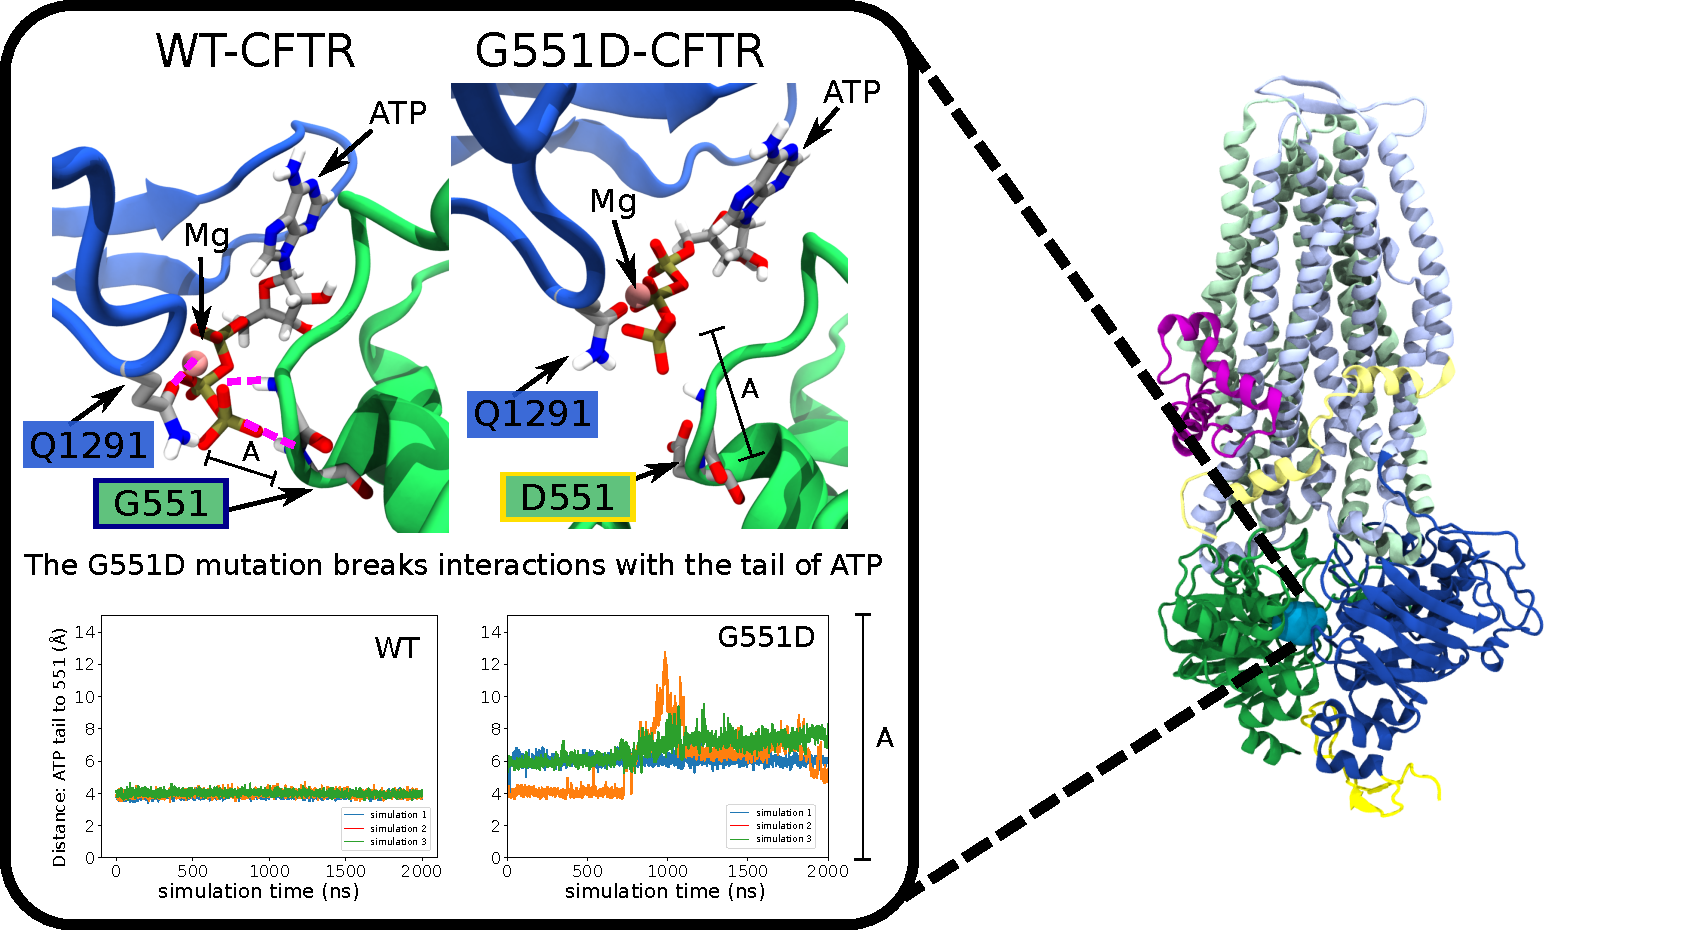
\includegraphics[width=\textwidth]{figures/perspective/G551D.pdf}
	\end{center}
\begingroup
\captionsetup{singlelinecheck = false, justification=raggedright}
\captionof {figure}[Pathogenesis in G551D-CFTR] {\textbf{Pathogenesis in G551D-CFTR}}{G551D-CFTR exhibits the prototypical gating phenotype \textit{in vitro} \cite{bompadre2007, wang2020}. A) The mutation is located on NBD1, in the vicinity of site 1, the hydrolytic ATP+Mg binding site. B) MD simulations indicate that this mutation disrupts ATP-binding, as the amide groups on the backbone of G550 and G551 stabilize the phosphate tail of the bound ATP molecule. These links were found to be disrupted in the mutant.} 
\label{G551D_results}
\endgroup

We will briefly continue the theme of previous chapters with a simple MD study to understand pathogenesis in a common gating mutation G551D. This will place the mutation in context with the rest of our work. This class III gating mutation occurs in NBD1 (Figure \ref{G551D_results}). It was the candidate for high-throughput screening in order to discover potentiator class drugs, as it is one of the most common gating class mutations \cite{vangoor2009,li1996}. This means that G551D is a good candidate for comparison  with other rare mutations, if we wish to guess which other mutations might respond to modulators in the same way.

In summary, G551D-CFTR disrupts the binding of ATP. In the next seciton we will demonstrate where this places the G551D mutation in relation to other mutations. 

\section{The Many Molecular Modes of Misfunction in CFTR}
It is unlikely that the course classification of 6 classes conventionally used to understand CFTR mutants can be used to theratype patients, a granular, molecular understanding will be needed to choose which mutations can be rescued by modulators, and we outline some computational studies which might be performed to help understand how this would work.

\begin{landscape}
\begin{figure}
	\begin{center}
	%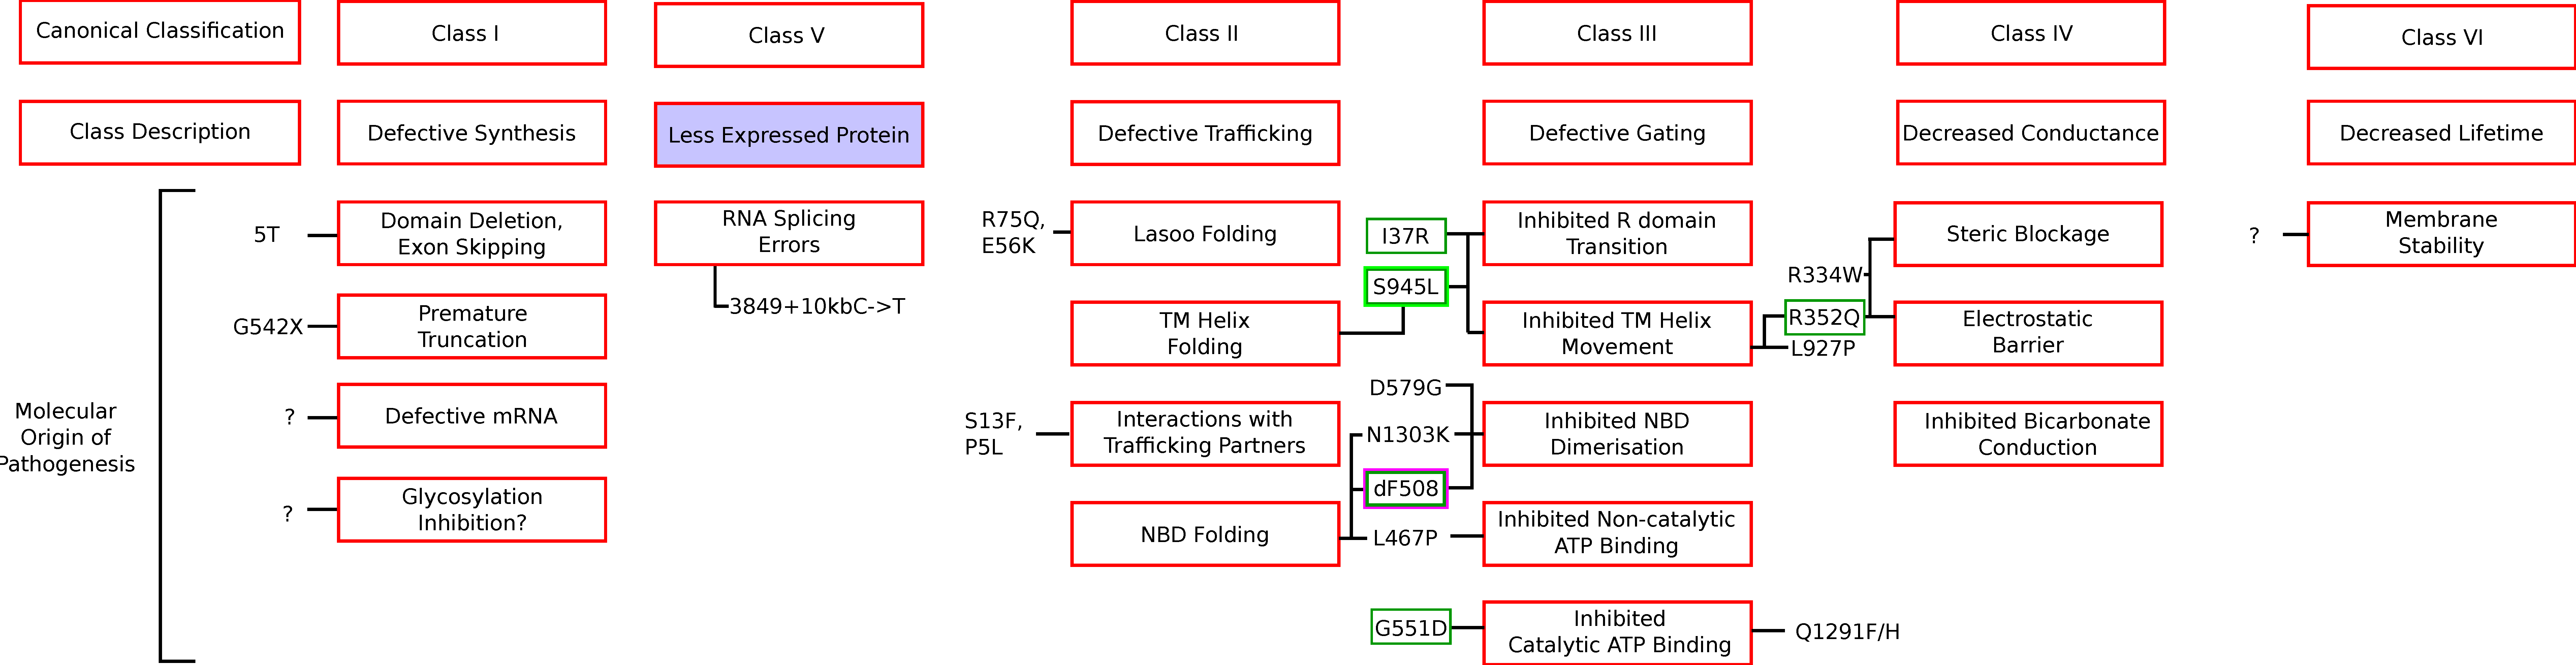
\includegraphics[angle=270,origin=c,width=0.38\textwidth]{figures/classes_mutations.pdf}\\
	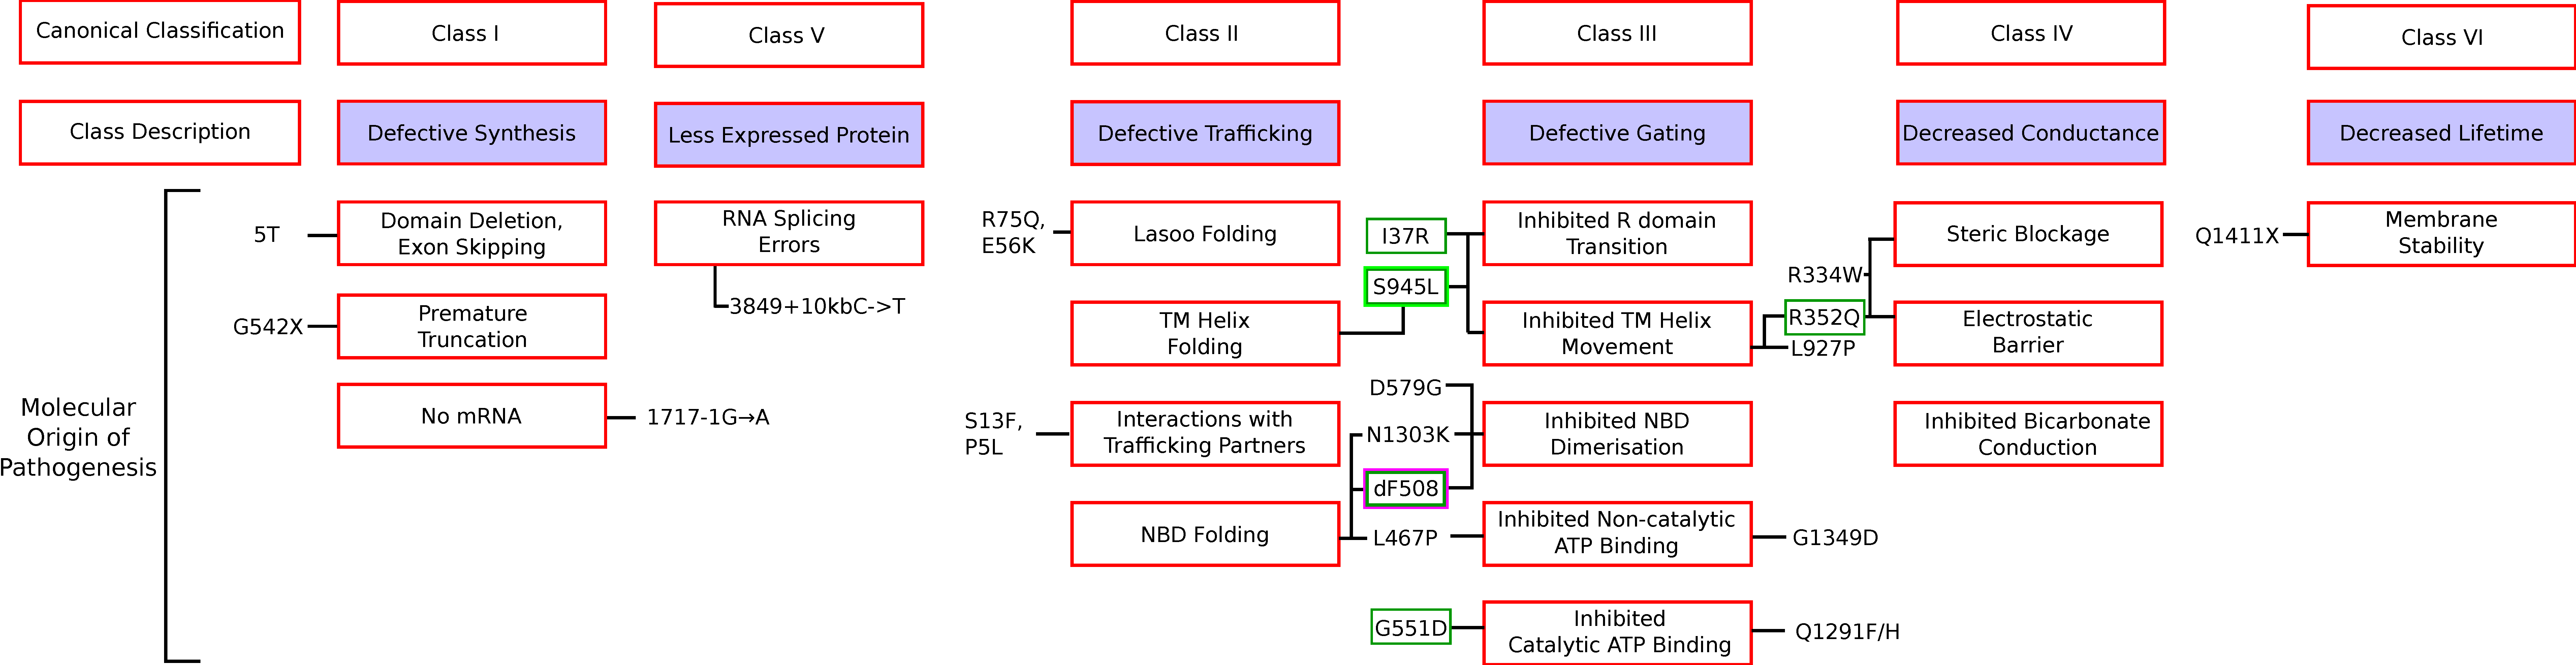
\includegraphics[width=1.5\textwidth]{figures/perspective/classes_mutations.pdf}\\
	\end{center}
	\captionsetup{singlelinecheck = false, justification=raggedright}
	\caption[Granular grouping of CF pathogenesis]{\textbf{Granular Grouping of Cystic Fibrosis Causing Mutations}{ Conventionally, molecular CF phenotypes are grouped into 6 classes. These classes, while useful in a clinic, are quite broad. They struggle to reflect that molecular misfunction of misfunction can arise from many interactions within CFTR. By realising that classification into a given class can be due to different factors we can gain a more complete picture of the molecular cause of CF by delineating the molecular fingerprint of each mutation. The links drawn in this figure arise from various places in the literature, alongside our own findings from this thesis and a generalised understanding of a mutation from its location on the CFTR protein, or from an analogous mutation \cite{bompadre2007, gong2004, wong2022, vangoor2009, vangoor2014, hoffmann2018, thelin2007, gene2008, trikafta_website, phuan2018, ensinck2022}.}
	}

	\label{granular_classification}
\end{figure}
\end{landscape}


\section{A Physics Motivated Approach to Precision Medicine in Cystic Fibrosis}
Obesrve in Figure \ref{granular_classification} how mutations which cause misfunction in lots of different ways respond to different modulators. In order to tie these results together, in this chapter I will propose a conceptual framework which explains how these drugs are able to treat such diverse molecular phenotypes. This model would appear to suggest that patients with rare missense mutations would be more likely to respond to respond to CFTR modulators. The implications of this model are also likely to inform the design of future generations of CFTR modulators. 

	\begin{center}
		\begingroup
	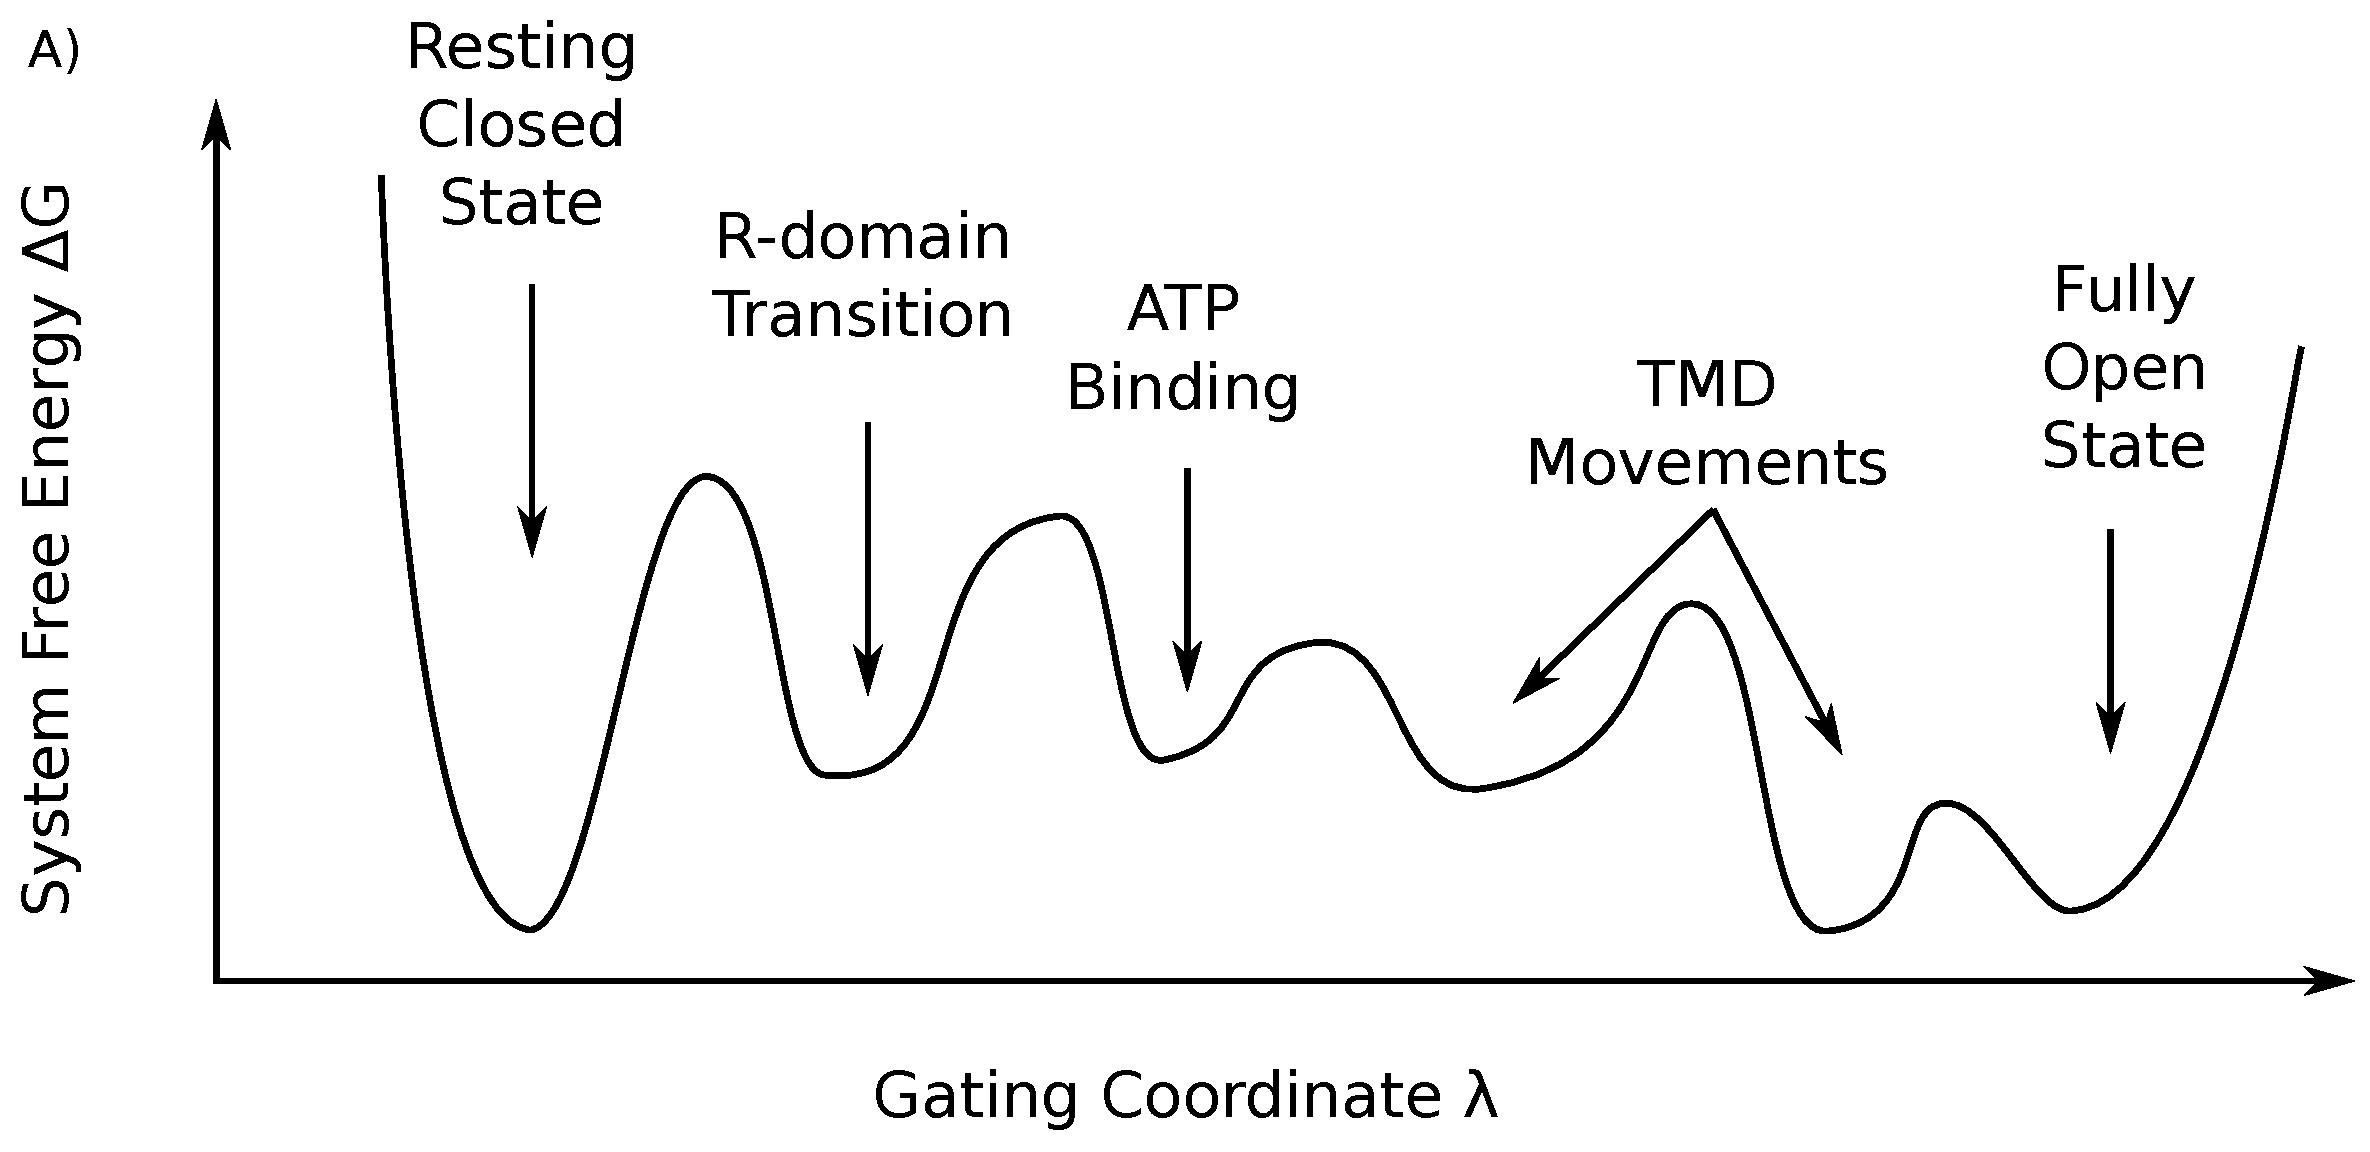
\includegraphics[width=0.8\textwidth]{figures/perspective/drug_landscape_1.pdf}\\
	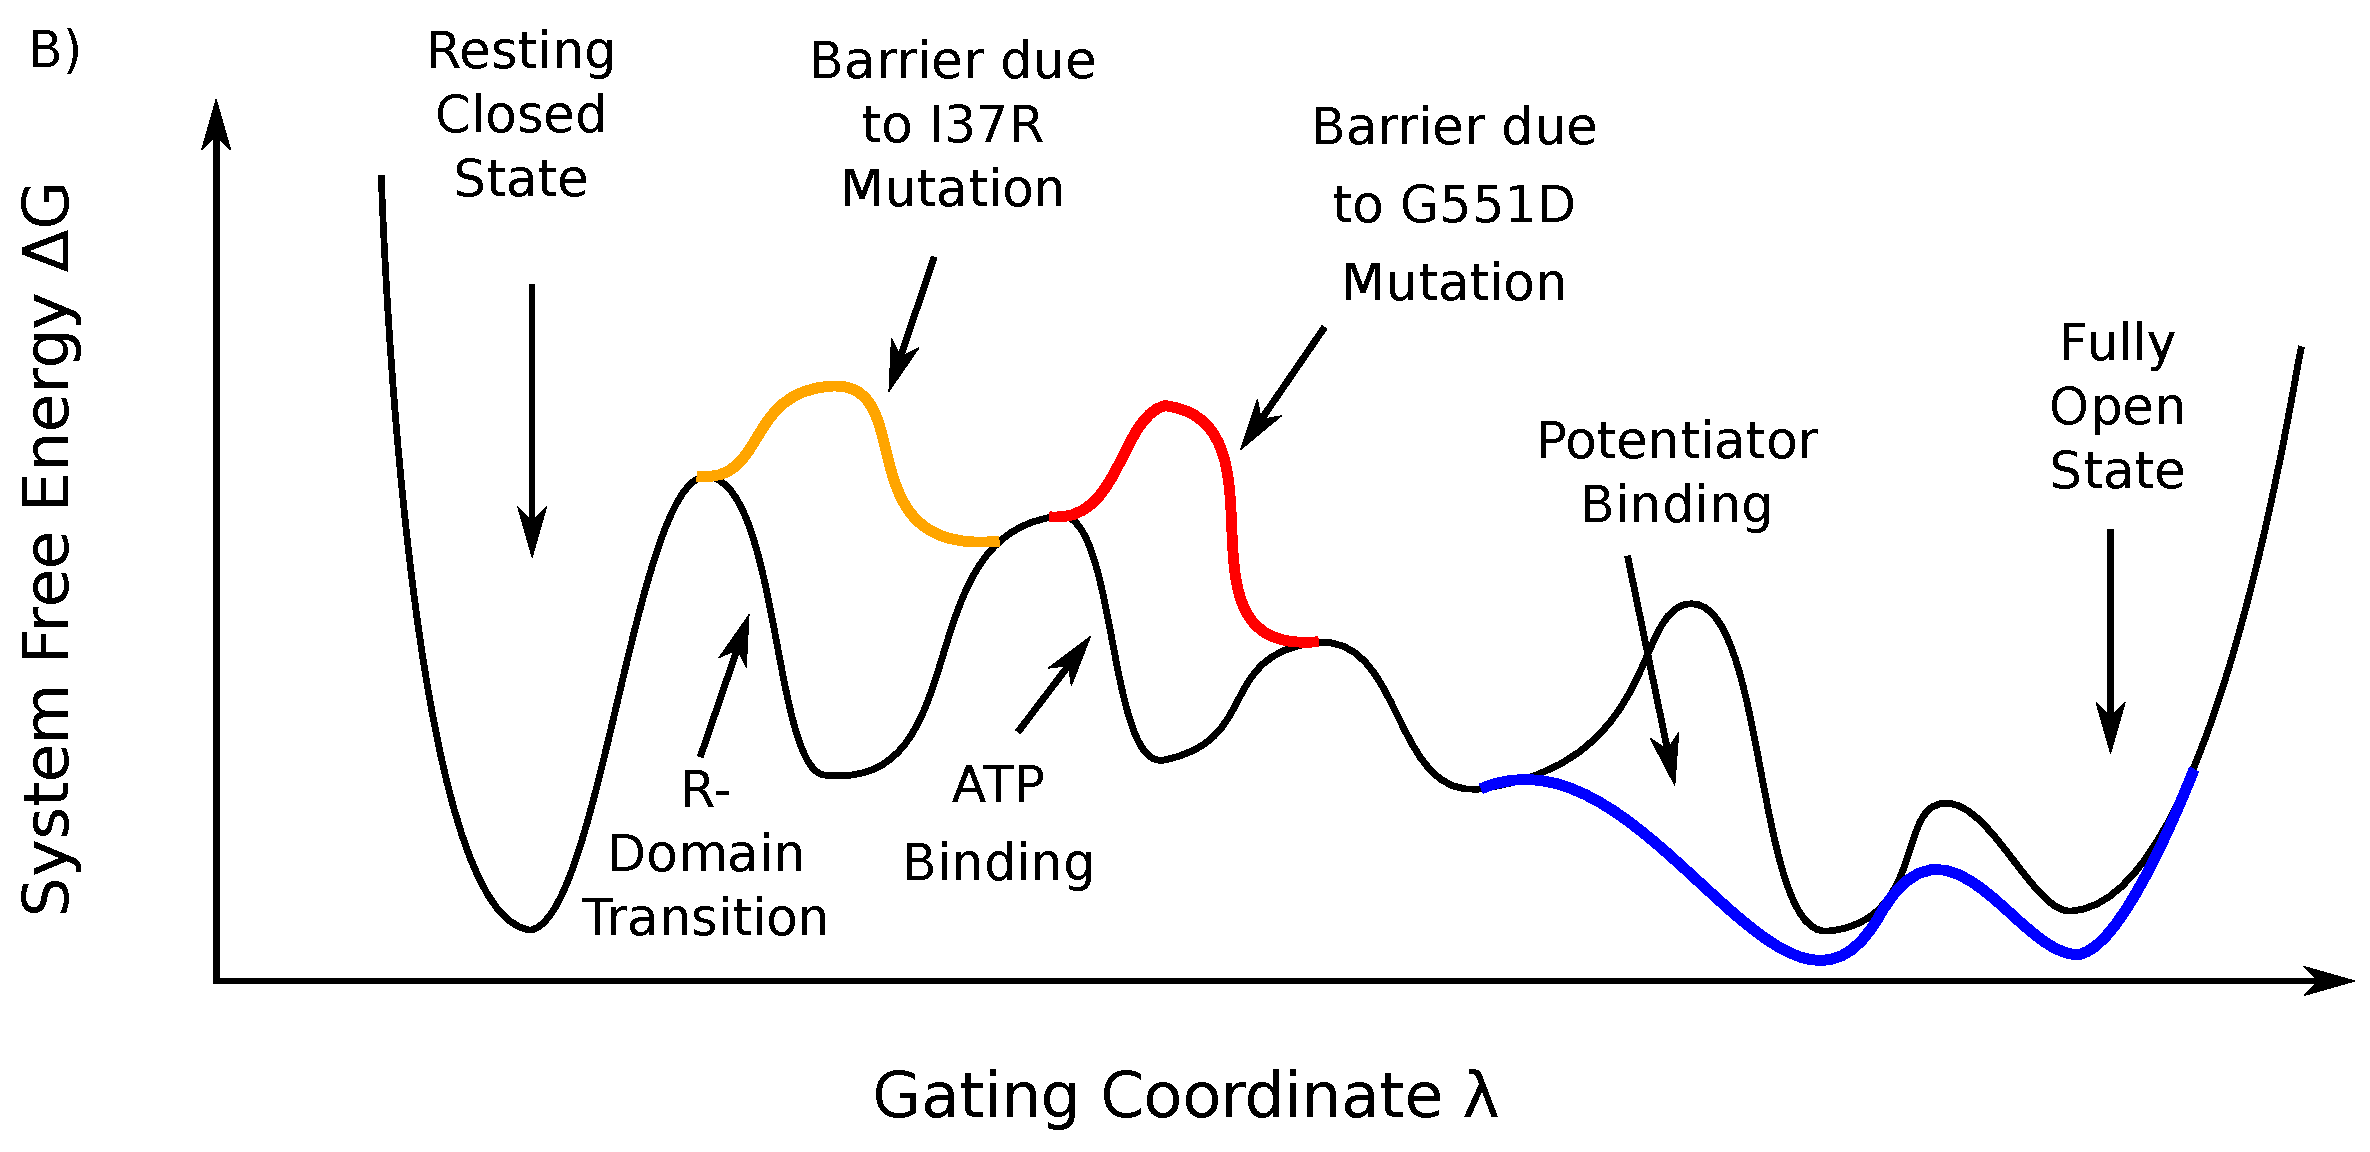
\includegraphics[width=0.8\textwidth]{figures/perspective/drug_landscape_3.pdf}\\
		\endgroup
	\end{center}
	\begingroup
	\captionsetup{singlelinecheck = false, justification=raggedright}
	\captionof{figure}[Conceptual Framework for the Pathogenesis of Mutations and The Action of Potentiators]{\textbf{Conceptual Framework for the Pathogenesis of Mutations and The Action of Potentiators}{ This model was produced to explain the apparent ability of CFTR modulators to treat rare mutations with a diverse set of phenotypes. A) The transition between the resting closed state and fully open state of CFTR can be visualised as a movement through an energy landscape. Along this transition various events must occur, such as the movement of the R-domain, ATP-binding and the rearrangements of the different domains of CFTR. Each of these events will have an energetic cost and payoff, giving rise to peaks and troughs in the free energy landscape of the transition. The relative heights of peaks and troughs here are for illustrative purposes only, but quantitative techniques to calculate them will have important implications for the treatment of CF and drug discovery. B) Gating class CF-causing mutations represent pathogenic barriers to this transition. They may arise in different parts of the energy landscape. For example, we have shown that G551D causes a disruption to the binding of ATP, while in chapter \ref{chap:I37R}, we saw a gating defect arise in I37R-CFTR from the misregulation of the position of the R-domain. This demonstrates how pathogenesis can arise in many different ways in CFTR. Furthermore, accompanying \textit{in vitro} studies of these mutations demonstrated that these unique mutations each respond to potentiator class modulators. This indicates that the action of potentiators is \underline{somewhere else} in this free energy landscape, relative to the perturbation caused by mutation. By understanding \textit{where} mutations are causing gating inhibition and \textit{how} drugs are accounting for the deleterious energetics, we can begin to build a molecular basis for the choice of modulators, tailored to particular patients.}}
	\label{drug_action_model}

	\endgroup


An analogous model could be drawn for the action of correctors. To do this we would need to clearly delineate the folding pathway of the CFTR protein and study how mutations cause aberrations in the folding landscape. Although work on this has begun \cite{krainer2018, kleizen2021, kleizen2020, fiedorczuk2022}, the folding pathway is much less straight forward to understand via simulations than the gating transition, so our proposed model will be detailed using the gating transition and potentiators.

The gating transition is simpler, as there are many easily measurable events which we can conceptualise, like ATP binding and pore formation. We will build our model with a focus on this aspect of protein function. Nonetheless, the concepts are transferable, to CFTR folding and as more corrector class drugs are developed and more mutant forms of CFTR are imaged we will gain more understanding f the folding pathway of this critical protein, so in time this model can be transferred to correctors as well. Additionally, as computer models improve we can simulate parts of this pathway as well. Computational capabilities are likely sufficiently advanced to simulate the full gating cycle of CFTR and so discover which parts of the landscape in figure \ref{drug_action_figure} are perturbed by mutations \cite{}. 

The above model in figure \ref{drug_action_model} gives a rational, physical basis for the wide range of molecular phenotypes that CFTR modulators appear capable of treating. This same model would appear to argue that we would expect most missense mutations we to respond to some sort of CFTR modulator. 

Currently a range of missense mutations are recommended for treatment by trikafta but many more are excluded from receiving this treatment due to a lack of testing. The above model suggests that when a patient carrying such a rare mutation does not respond to modulator therapy, it is unlikely that the lack of a response is due to the inability of these modulators to rescue the function of CFTR. From the perspective of protein physics, $\Delta$F508 is likely to perturb the protein much more than most missense mutations \cite{}. Rather, it is more likely that if a patient does not respond to modulators it is due to the broader heterogeneous response to modulators found in all CF patients \cite{}. 


\section{The Poorly Studied Mutation Q1291H has a Similar Effect to G551D}

Through our molecular modelling we noticed another defect, Q1291H appears to produce a similar molecular defect to G551D even though it affects a different domain of CFTR (NBD2 as opposed to NBD1). G551D is much more common than Q1291H, and so patients carrying the former may access potentiators. However, Q1291H is extremely rare, so rare in fact it has not been well described clinically, with only 30 CFTR alleles with this mutation recorded in the CFTR2 database \cite{cftr2}. Samples with this mutation are in the biobank of Sydney Children's hospital, taken from a CF afflicted patient. 

Because of their heterozygous alleles, and the rarity of the Q1291H mutation, this patient is currently excluded from receiving modulator therapy. Although computational modelling is not sufficiently advanced to make a recommendation for this patient without \textit{in vitro} studies, this situation is common for those carrying rare forms of CF. Hence, we have undertaken computational modelling in order to understand the molecular defect caused by the Q1291H mutation. Our modelling would lead us to believe that there is a high likelihood that cells carrying the Q1291H mutation would respond to potentiators or a combination therapy. 

These conclusions are motivated by the observation that both the prototypical gating defect caused by G551D and Q1219H cause a disruption to the binding of ATP at site 1. The latter .  

The preceding chapters have given technical and molecular details about the cause of Cystic Fibrosis by rare genetic mutations, and further demonstrated that these mutations may be treated by existing small molecule drugs. The unique molecular fingerprint of each mutation indicates that in order to deliver better outcomes to patients a more personalised approach is necessary in the choice of medication. 


%There is no reason to beleive that even in patients who do not show benefit from modulator therapy that the drugs are for some reason not reaching the CFTR protein. In fact, they seem to metabolise the drugs at teh same rate as patients who do. The success of preclinical models indicates that the problem is the cellular level and not at the level of organs or tissues. There is probably some genetic or cellular component that has not yet been identified which, once addressed, could bring the benefits of modulators to these patients.




\begin{figure}
	\begin{center}
		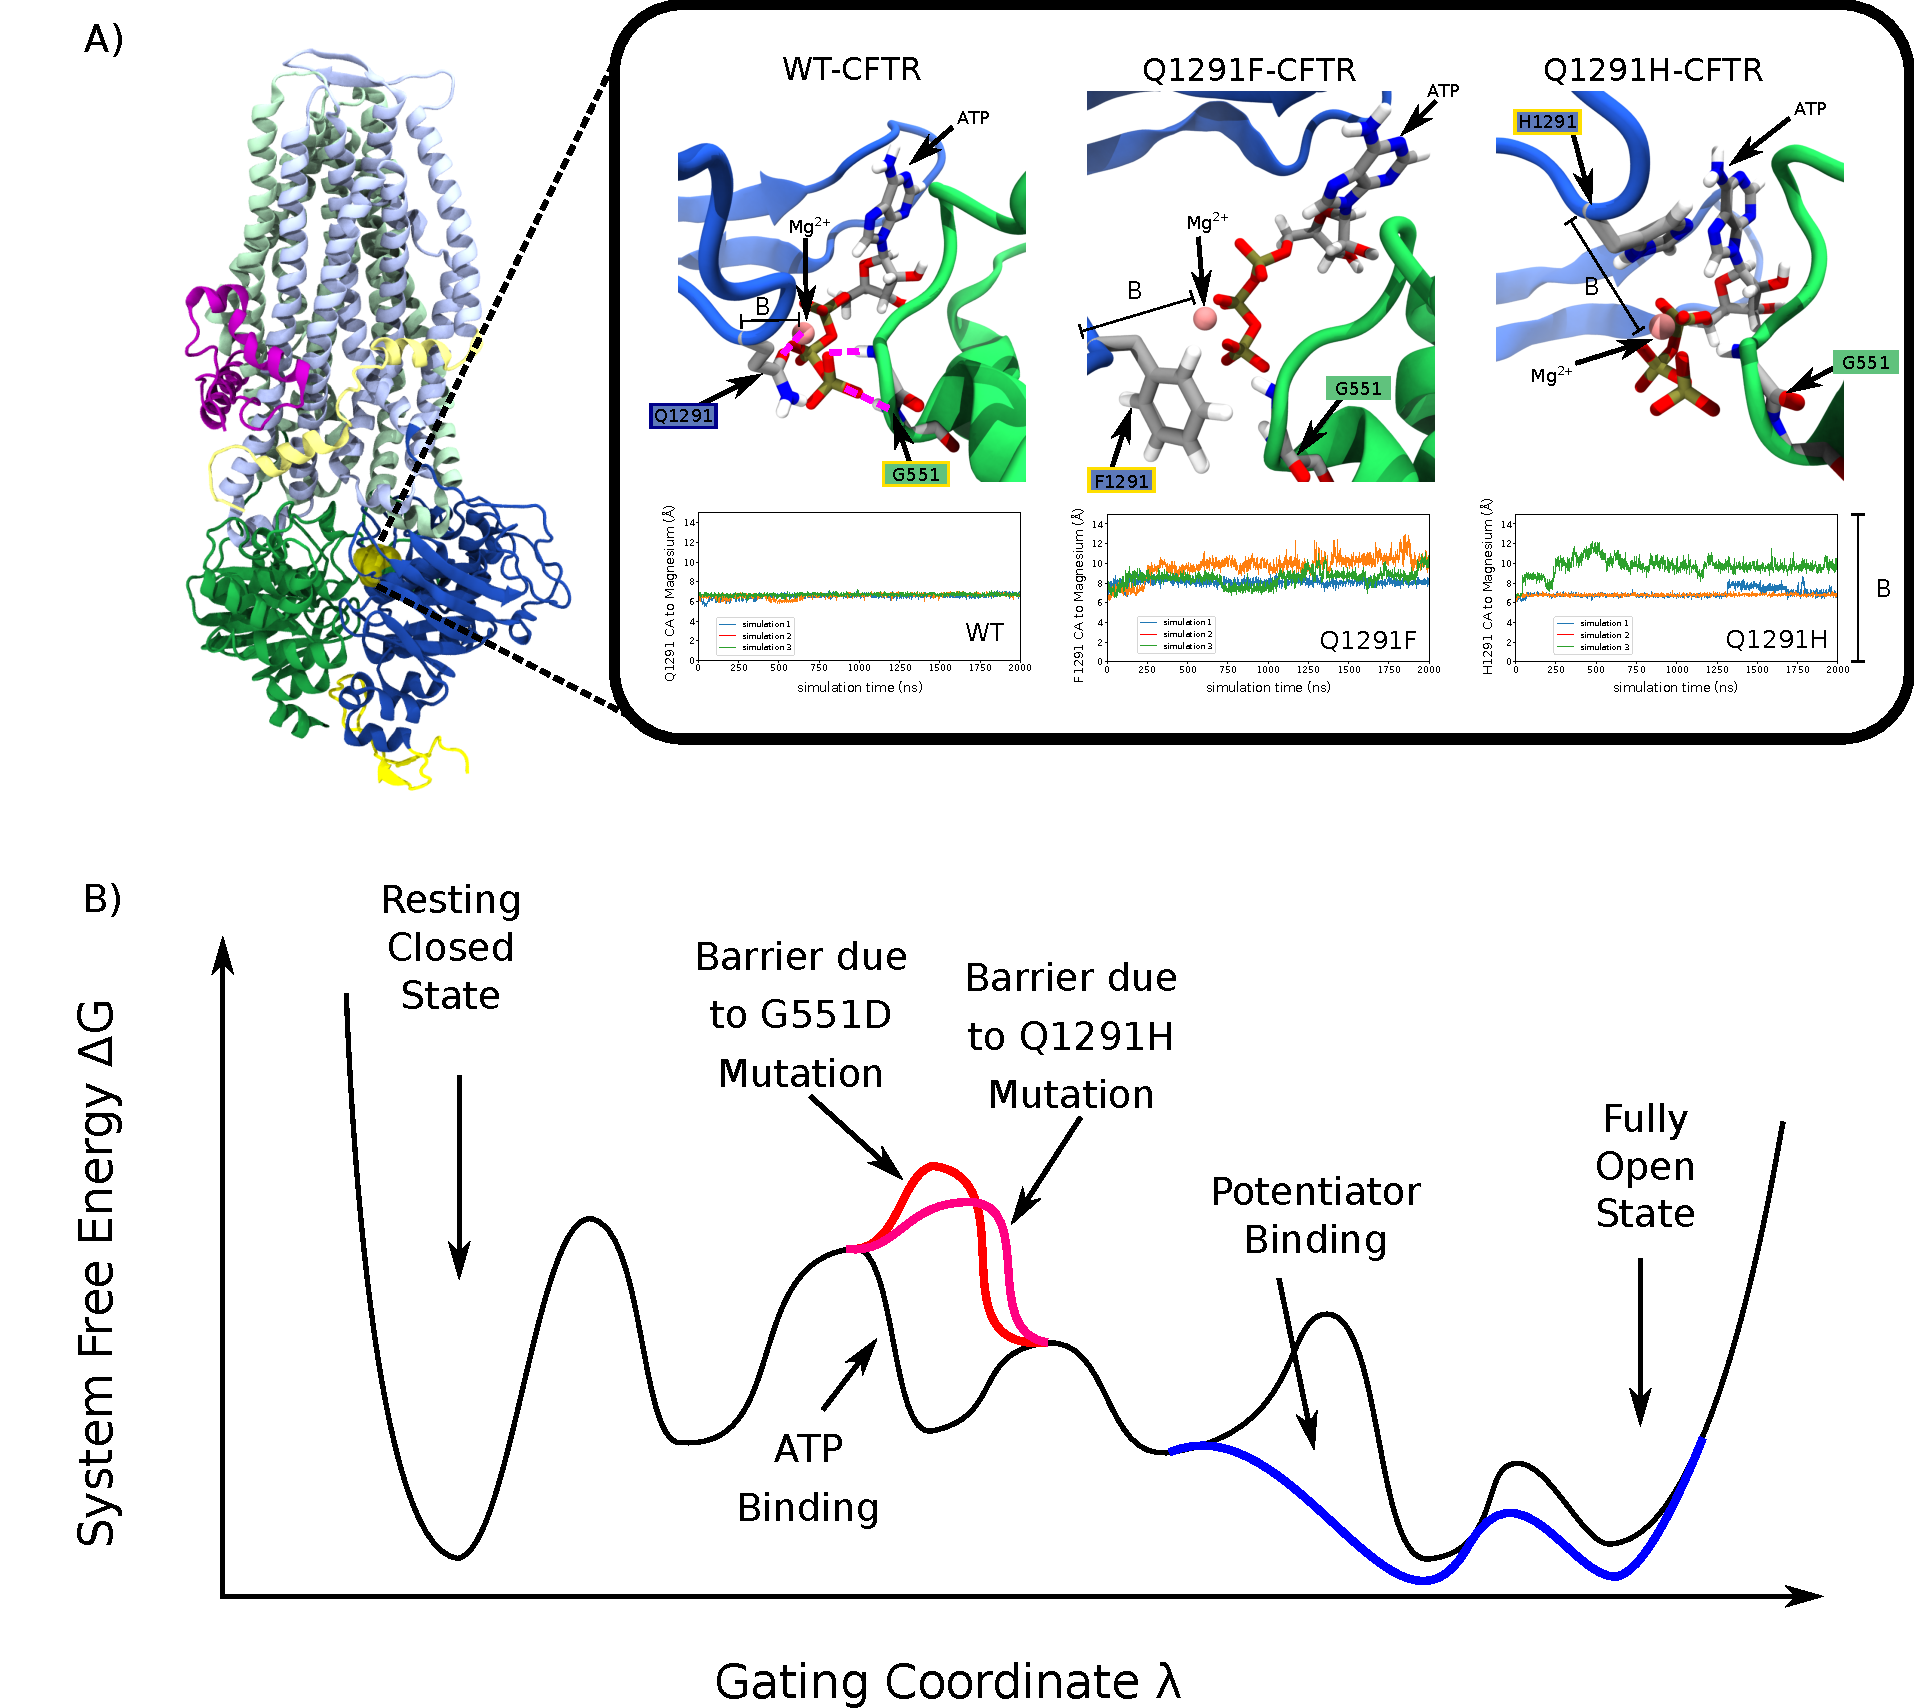
\includegraphics[width=\textwidth]{figures/perspective/Q1291.pdf}
	\end{center}
	\captionsetup{singlelinecheck = false, justification=raggedright}
	\caption[Pathogenesis in Q1291H-CFTR]{\textbf{Pathogenesis in Q1291H-CFTR}{A) The Q1291H mutation occurs on NBD2, in the vicinity the catalytic ATP binding site. B) It appears as though this mutation also causes disruption to the binding of this ATP molecule, much like G551D. Data from simulations Q1291F is also included, as it more reliably produces the molecular perturbation which we expect is characteristic of the Q1291H mutation. \textit{In vitro}, the two mutations produce similar behaviour and this is confirmed in our simulations. }}

\end{figure}


%These drugs are clinically efficacious \cite{VanGoor2014} on several mutants with some curious exceptions like N1303K. I suggest the following mechanism for their action. I suspect a similar analogy exists for the action of the correctors. WT-CFTR exhibits a natural landscape with kinetic barriers in the transition between the closed and open states. A gating class mutation to CFTR will introduce a kinetic barrier in the pathway of this conformational transition. What these drugs do is reduce a barrier in the existing conformational landscape of CFTR. This compensates for the barriers introduced by the mutation. j


\section{Summary}
In summary, the important findings from the 4 prior modelling studies, and the presented study of G551D have lead us to propose a model for the rescue of gating class mutations by small molecule drugs. This model sought to account for the fact that we have seen 5 unique defects all respond to potentiator drugs, and we expect a similar model could be drawn for folding class defects. This that many disease causing alleles will respond to modulator therapy, even though they are currently excluded from these treatments by regulatory agencies. 

In recent years there have been a slew of rare CF-causing genotypes discovered in populations with low rates of Cystic Fibrosis compared to Caucasians. These genotypes from Asia and the Middle East are often ultra-rare leading, to poor outcomes for these patients \cite{}. 

In order to collect further evidence to support this conclusion and translate these findings into clinical practice, in the next chapter we will outline priorities for future \textit{in silico} and pre-clinical studies into the function of CFTR.
